Object detection has become an essential part of many fields such as medical imaging, transportation, or industrial safety monitoring. Despite its wide range of applications, object detection is still one of the most challenging and fundamental problems in computer vision \cite{object_detection_20years}. Modern deep learning-based object detectors that automatically localize and classify objects of interest in images are only as good as the data used for training the model. Depending on the application, training an accurate model might require thousands to even millions of diverse images \cite{optimalmedic, Kuznetsova_2020}. As collecting large-scale datasets can be time-consuming and expensive, data scarcity might become a bottleneck in training accurate object detection models if no public datasets are available. Especially in fields such as military, medical, or surveillance imaging, data gathering can be difficult due to privacy concerns, rare occurring events, or the sheer difficulties of capturing images \cite{akrout2023diffusionbaseddataaugmentationskin,tanks,app14114558, math11224588}.

The traditional approach to overcome data scarcity is to use data augmentation techniques, where existing images are modified using operations such as rotation, scaling, or flipping to create new training images \cite{10084010}. While traditional data augmentation methods can help improve model robustness, they are limited to producing variations of the original image, bringing nothing new. In this work, methods are utilized that the author refers to as "augmentation with steroids," as they can produce images with new content through synthetic data generation from fine-tuned text-to-image models.

The release of ChatGPT at the end of 2022 started a surge of AI hype. Around the same time, generative text-to-image models such as DALL-E 2, Midjourney, and Stable Diffusion also gained a lot of attention for their ability to generate high-quality images that mimic various artistic styles and create realistic pictures from text prompts \cite{Chen2023GenerativeAL, Reben_2022}. The quality of these models has developed to the point that it can be very difficult to distinguish them from real-world photographs \cite{kamali2025characterizingphotorealismartifactsdiffusion}. In addition, there are open-source models that have enabled users to fine-tune large-scale generative models to produce images that reflect the content of their training datasets. While text-to-image generative models have raised ethical concerns, including privacy violations, unauthorized use of artistic styles, and the spread of misinformation, they also present promising opportunities in many fields such as education, healthcare, and object detection \cite{bird2023typologyrisksgenerativetexttoimage, Sudha_Aruna_Sureka_Niveditha_Prema_2024}. By applying these models to object detection, it is possible to synthesize diverse datasets that generalize to different content while capturing visual similarities to the target images, even creating new scenarios that were not in the original dataset. This work will investigate the potential of the text-to-image model to address data scarcity by increasing both the size and diversity of the dataset and how it may help with class imbalance in edge cases.

\begin{figure}[htbp]
    \centering
    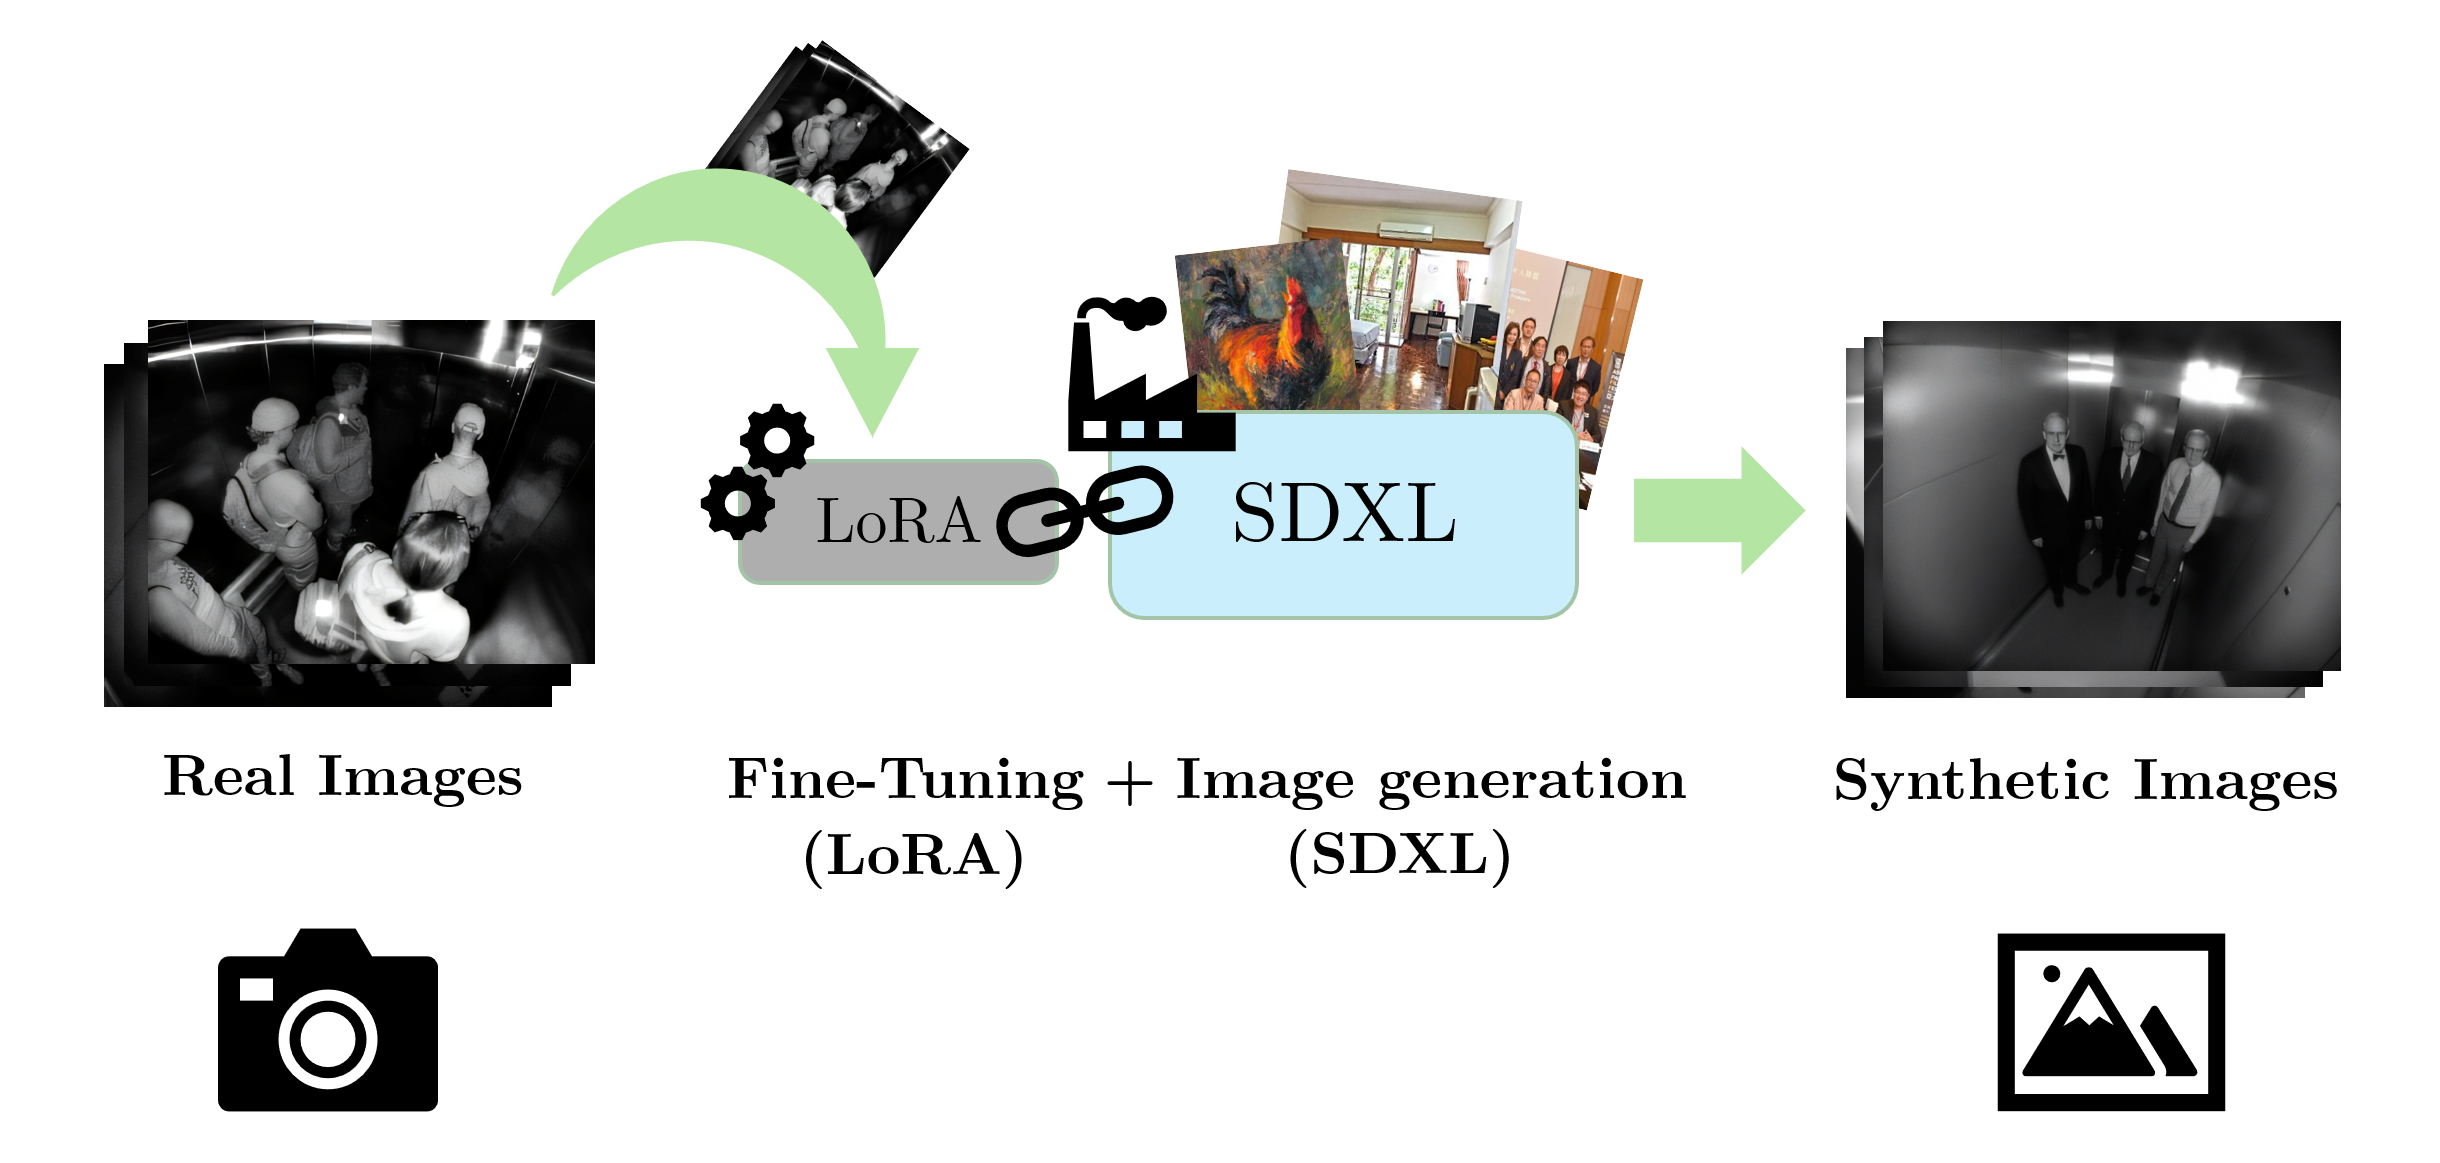
\includegraphics[width=1\textwidth]{images/intro3.png}
  \caption{Illustration of the synthetic image generation process. Captured sensor images are used to train a LoRA model, which is then used to fine-tune the SDXL text-to-image model. Because SDXL is trained on large-scale datasets of captioned images, the fine-tuned model can generate diverse images from text prompts that resemble the sensor images when the LoRA is applied.}
    \label{fig:intro}
\end{figure}

The research question of this work is formulated as follows: Can synthetic images generated from a fine-tuned diffusion-based text-to-image model improve the performance of an object detection model? To answer this question, an end-to-end pipeline for synthetic data generation and object detection is implemented from scratch. The work focuses on detecting people in near-infrared sensor images captured in small indoor environments. By using 31 images captured from the sensor, the Stable Diffusion XL (SDXL) text-to-image model is fine-tuned using low-rank adaptation (LoRA) to generate synthetic images that resemble the sensor images. To evaluate the effectiveness of synthetic images in improving object detection performance, multiple YOLOv8n object detection models are fine-tuned using different combinations of real and synthetic images.

This work is structured as follows: Chapter~\ref{ch:background} provides an overview of the related work in the field of object detection and synthetic data generation. Chapter~\ref{ch:methodologies} details the scope of this work and the implemented end-to-end pipeline for synthetic data generation and object detection. Chapter~\ref{ch:results} presents the results of the trained fine-tuned object detection models. Chapter~\ref{ch:discussion} discusses the implementation and results, and suggests recommendations for implementations and future work. Finally, Chapter~\ref{ch:conclusion} concludes the work with a summary of implementations and results.


%Caption. Text-to-image models are capable of generating high-quality images from text prompts, mimicking 


%The synthetic images are generated by fine-tuning a diffusion-based text-to-image model using a small set of real images with bounding box annotations. The generated synthetic images are then combined with real images to train an object detection model based on the YOLOv8 architecture. The performance of the object detection model is evaluated using different combinations of real and synthetic data to analyze the impact of synthetic images on model accuracy.
%The goal of this work is to evaluate whether synthetic images generated with diffusion-based text-to-image model can improve the performance of an object detection model.
%The thesis has three main objectives:
%1. Reviewing existing methods to generate synthetic images and their effectiveness to improve performance of object detection models and selecting one method for implementation.
%2. Implementing from scratch a complete synthetic data and object detection pipeline.
%3. Analysing the effect of different combinations of real and synthetic data on the performance of the object detection model and mirroring results from the literature. 
%Chapter 2 is divided three main topics. First, the theoretical background about object detection and deep learning. Second sim-to-real problem and third text-to-image models.


%This opens new possibilities to use that scarce data to fine-tune text-to-image models and generate synthetic images that resemble real images. As model can change various aspects of the generated images, quantities of objects, environment or clothes of people ... with a text prompt. ... So giving it a nickname "augmentation with steroids".

%In modern world object detection has become an essential part of many applications such as medical imaging for detect cancer or even detect detect fruits from refrizirator.

%With it there is possibility to transform data distribution of other images to match target domain. 

%Object detection is one of the most fundamental yet challenging problems in computer vision. Modern approaches to localizing and classifying objects in images rely on deep learning, where an object detection model is trained to recognize objects of interest. Training such a model requires, depending of application, thousands to millions of images a lot of diverse data \cite{ANDVAAG20240268,app14114558}. In addition a model trained by insufficient amount of data usually suffers from overfitting, where the trained object detection model does not detect objects on unseen data, but just on training data \cite{agrawal2024syn2realdomaingeneralizationunderwater}. It's said that one of the challenging problems in training modern object detection model is the data scarcity \cite{zhu2024odgendomainspecificobjectdetection}. Sometimes it's hard to collect own data records due time or cost if there is not excisting datasets \cite{kiefer2021leveragingsyntheticdataobject}. Not it is very hard collect images in general but also in the field of medical, industrial or aerial imaging there might be other difficulties to collect data like privacy issues, rare occuring events or difficulties to capturing images \cite{app14114558, akrout2023diffusionbaseddataaugmentationskin,tanks,app14114558, math11224588}.

%Because objects of interest can appear differently depending on context, like due deformability, occlusion or viewpoint, it can be very laborious to collect diverse set of training images. This is  common especially cases where there is scarcity of existing datasets. One usual way to increase the size of training data from already taken images is to use data augmentation, where different transformations like rotation, translation, or scaling are applied to the image \cite{9531849, zoph2019learningdataaugmentationstrategies}. Even though this helps make the object detection model more robust, it is limited to only utilizing existing data. To increase the size and diversity of a small dataset also bringing something new, it can be done by synthesizing data \cite{nguyen2024application, 9564932}.

%To generate synthetic images, methods like 3D simulations, image blending, or image generation by text-to-image models are mainly used. One advances of using synthetic data is controlability and customization \cite{10484172}. These are usefull features for hightening diversity of the dataset but also to create images inclusing rare or ignored objects and scenarios \cite{9564932}. Depending on the method used, it can create a great amount of diverse images quickly and possibly automatically labeling them \cite{9377353, Bartolovic2024FromST}. However, there is still an existing difference between similarly created and real images. The synthetic-to-real (or simulation-to-real) gap describes how different real and synthetic domains are \cite{mishra2024closingvisualsimtorealgap, agrawal2024syn2realdomaingeneralizationunderwater}. As synthetic images differ from real images, sometimes in cases where only synthetic data is used in training, the model is not able to detect objects from real data, but using synthetic data together with real data in training helps improve the model \cite{Bartolovic2024FromST}. However, modern text-to-image models can generate more and more realistic images that can be very hard to distinguish from real images without a separate AI model to recognize them \cite{anon2024detectingundetectablecombiningkolmogorovarnold, kamali2024distinguishaigeneratedimagesauthentic}. With fine-tuning, a text-to-image model can generate images that mimic different art styles, new objects, or even different scenarios \cite{smith2024loradiffusionzeroshotlora}.








